\section*{\LARGE Appendix}
\counterwithin{figure}{subsection}
\renewcommand{\thefigure}{\thesubsection.\alph{figure}}

\section{Robustness checks}
\subsection{Different definitions of effective tax rate}
\label{appendix_itrc}

\begin{figure}[!ht]
\centering
\includegraphics[width=0.9\textwidth]{"images/18-09 itrc_comparison"}
\caption{Mean of implicit tax rates on consumption for each country.}
\label{fig:itrc_comparison}  
\end{figure}

There are three main definitions for computing implicit effective tax rates on consumption in the economic literature, as described in \cite{euro2016taxation, mendoza1994effective, carey2000average}. We draw on those works in order to propose the following definition:
\[ \tau_{c,y} = \frac{consumption\ taxes\ revenue}{C - CGW - R } \]
where $consumption\ taxes\ revenue$ includes all revenue from consumption taxes, including value-added-taxes (or sales taxes if applicable), excise taxes, taxes on specific services, etc. $C = CP + CG$ is the total final consumption expenditure (private consumption and consumption of general government). $CGW$ is the amount of wages of employees paid by general government, and $R = R_{actual} + R_{imputed} =$ are actual and imputed rentals for housing.

The different possible definitions of implicit tax rates rely on different definitions of the taxable consumption. For example, the definition in \cite{euro2016taxation} relies on a narrower taxable basis, constituted only of private consumption
\begin{equation}
    \label{itrc_euro}
    \tau_{c,y} = \frac{consumption\ taxes\ revenue}{CP}
\end{equation}
while the definition in \cite{carey2000average} considers a broader definition, by taking all consumption
\begin{equation}
    \label{itrc_carey}
    \tau_{c,y} = \frac{consumption\ taxes\ revenue}{C}
\end{equation}

The choice of removing or not rents from the denominator depends on the definition of taxable consumption in micro-data. Since we account for the fact that rents are not subject to consumption taxes by removing rents from the micro-data on consumption, we subtract rents from the denominator of the implicit tax rate. If we do the same for the two alternative definitions described earlier, our definition of implicit tax rates on consumption is thus structurally bounded above by the tax rate under definition \eqref{itrc_euro} and below by that under definition \eqref{itrc_carey} (see \cref{fig:itrc_comparison}). These alternative definitions can be used to produce robustness checks.

\subsection{Estimated regressivity is mitigated when taking rents into account}
\label{sec:rents}
\begin{figure}[!h]
\centering
\includegraphics[height=0.4\textheight]{"images/18-11-18 total_nonrent_propensity fr10"}
\caption{Rents represent a higher share of consumption at the bottom of the income distribution (France 2010)}
\label{fig:total_nonrent}  
\end{figure}

Our method allows to account for the fact that housing rentals are not subject to consumption taxes. They are an important part of households' consumption, and they represent a higher share of consumption for poorer households (\cref{fig:total_nonrent}). As a result, the downward slope of propensities to consume are less pronounced when rents are removed from the total amount of consumption. Therefore, we can conclude that micro-simulation methods which apply tax rates on the whole consumption (rent or not) are slightly overestimating the regressivity of consumption taxes.

In order to maximize our coverage of countries and years, we also define another version of the effective tax rate, where actual rentals are not removed from private consumption at the denominator. This definition will be used when micro-data on consumption is not separable between rentals and the rest of the consumption. This smaller rate will be applied on a bigger amount of consumption.
\[ \tau_{wr}= \frac{consumption\ taxes\ revenue}{CP - R_{imputed} + CG - CGW}\]

As shown in \cref{fig:kakrent}, estimated regressivity is reduced when rents are taken into account, and removed from the amount of consumption: the absolute value of the Kakwani index of regressivity can be reduced by up to 20\% for some countries.

\begin{figure}
\centering
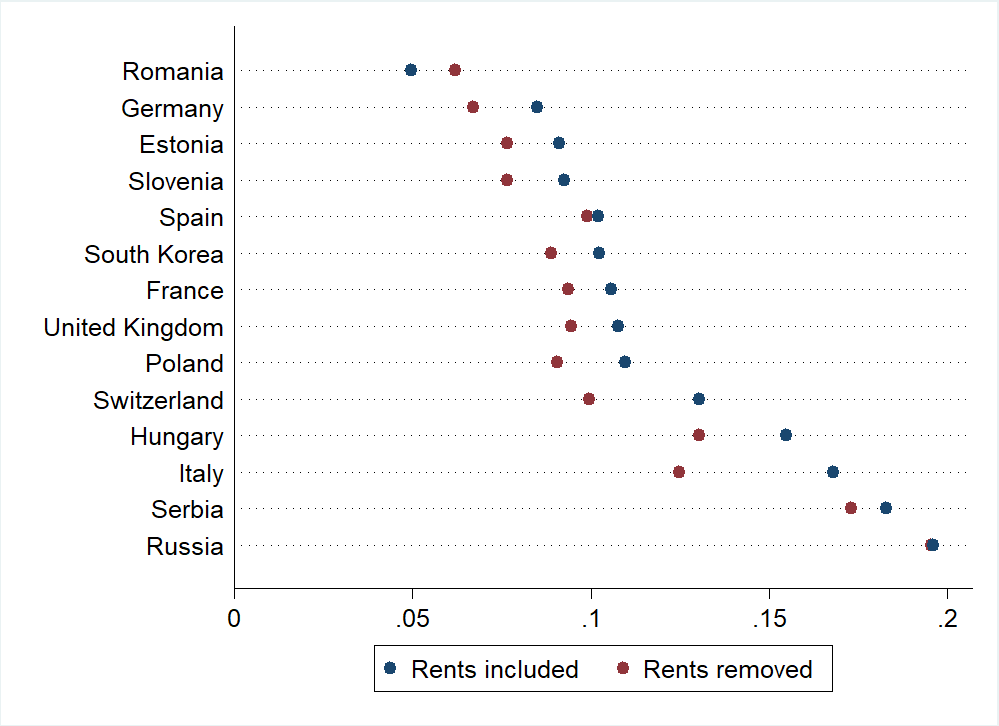
\includegraphics[width=0.9\textwidth]{images/18-03-18_kak_kak_wor_mean}
\caption{\label{fig:kakrent} Mean value of Kakwani index whether taxable consumption includes rentals}
\end{figure}

\subsection{Imputation error on consumption depending on the model}
\label{sec:compare_models}
\Cref{fig:compare_models} shows the R2 coefficient for 57 countries-years where imputed and observed values of consumption can be compared. Out of the 57 country-years for which we impute consumption both with \eqref{equ:mod1} and \eqref{equ:mod2}, we observe that model 2 increases the explained variance for 54 of them. On average, it is increased by 33\%, as measured by the R2 coefficient. Overall, the R2 coefficient for model 2 is 0.45 on average, being larger than 0.36 for 75\% of country-years, and larger than 0.56 for a quarter of our observations.

This shows that the independent variable ``cost of housing'', which is the main difference between the two models, provides significant additional information for the imputation of the households' consumption.

\begin{figure}[!h]
\centering
\includegraphics[width=\textwidth]{"images/19-04-05 R2 compare models"}
\caption{Explained variance in the two models for various countries}
\label{fig:compare_models}  
\end{figure}


\subsection{Prediction error for redistributive impact}
\label{sec:imputation_error}
The imputation model produces reliable estimates of post-tax Gini coefficients.
\begin{figure}
    \centering
    \includegraphics[height=0.45\textheight]{"images/19-02 prediction error ours mod2"}
    \caption{Actual and predicted Gini coefficient of post-consumption-tax income}
    \label{fig:prediction_error}
\end{figure}

\section{Decomposition of redistributive effect}

\subsection{Vertical and horizontal redistribution}
\label{sec:decomposition}
Effective redistribution can be decomposed into vertical redistribution, measured by the Reynolds-Smolensky index ($RS$), and horizontal redistribution, measured by the reranking index ($Re$):
\begin{equation}
 \label{equ:g_diff}
    \Delta G = G_{dhi} - G_{dhi-tax}  = RS - Re
\end{equation}

Vertical redistribution relates to the amount of tax that is distributed in a progressive or regressive way related to income. A measure of vertical redistribution, the Reynolds-Smolensky index, is defined as follows [reference à ajouter]:
\[ RS = G_{dhi} - C(dhi-tax, dhi) \]
where $G_{dhi}$ is the Gini index of the pre-tax income, while $C(dhi-tax,dhi)$ is the concentration index of the post-tax income ordered on the pre-tax income. This term is thus relatively close to the Gini index of the post-tax income.

Horizontal redistribution is the amount of redistribution that is orthogonal to the distribution of income. The reranking index of horizontal redistribution is a measure of the amount of redistribution that is not due to the regressivity of the tax, but rather an inequality that is created between individuals in the same range of income. It is defined as follows:
\[ Re = G_{dhi-tax} - C(dhi-tax,dhi) \]

By definition, the reranking $Re$ is non-negative, so by \cref{equ:g_diff} the Reynolds-Smolensky index is an upper bound for effective redistribution, and it is a measure of the maximum reachable redistribution if no reranking was entailed by consumption taxes. In our case, if redistribution is negative, then the RS index is a lower bound for the anti-redistributive effect (in absolute value). The rise in income inequality due to taxes is thus the sum of the vertical anti-redistribution (due to the regressive pattern) and the reranking due to the variation in propensities to consume between households of same levels of income. In practice, the Reynolds-Smolensky index is close to the difference in Gini coefficients (see \cref{fig:reranking}): the reranking generally accounts for less than 20\% of the redistributive impact. 

\begin{figure}
    \centering
    \includegraphics[width=\textwidth]{"images/19-02 decomposition effective redistribution"}
    \caption{Decomposition of redistributive effect}
    \label{fig:reranking}
\end{figure}


\subsection{Kakwani indices of regressivity}
\label{sec:kakwani}

We have seen in \cref{equ:decomp_RS} that the vertical redistribution operated by consumption taxes can be viewed as the product of two independent terms: the regressivity, a micro-level term linked to propensities to consume decreasing with income, and the rate of consumption taxes, a macro-level term.

We use the Kakwani index as an index of regressivity of consumption taxes. This indicator is a measure of how concentrated taxes are on one end of the income distribution or the other. It is equal to the difference between the concentration index of the tax relatively to (pre-tax) income and the Gini coefficient of the income [référence à ajouter]. Namely:
\[ Kakwani(tax, dhi) = C(tax,dhi) - Gini(dhi) \]

The concentration index $C(tax,dhi)$ is a measure of how much the distribution of the tax payments is skewed towards highest incomes. The range of its values is [-1;1], -1 indicating that all the tax payments are concentrated on the one poorest individual, while 1 indicates that all the tax payments are concentrated on the richest individual. The computation of this concentration index does not take into account the level of initial income inequality. By substracting the Gini index of income, the Kakwani index provides simple information, based on its sign: if the Kakwani index is positive, it means that the tax payments are more heavily concentrated towards the highest percentiles of income than income itself, meaning that the tax is progressive. On the contrary, if the Kakwani index is negative, then the distribution of tax payments is less skewed to the right than the distribution of income, meaning that the tax is regressive. We are thus expecting negative Kakwani indices.

For one fixed tax rate, we can make assumptions on the Kakwani index and thus have a range of possible RS index values. When the Kakwani indices are derived from imputed consumption values, this will be useful to provide lower and upper bounds on the possible RS values.

We compute the Kakwani index for all the datasets where consumption data is available (i.e.\ 77 country-years), the results are summed up in \cref{fig:kakwani_boxplot}. Approximately half of Kakwani indices lie between -0.10 and -0.15, while almost all of them lie between -0.05 and -0.20.
\begin{figure}
    \centering
    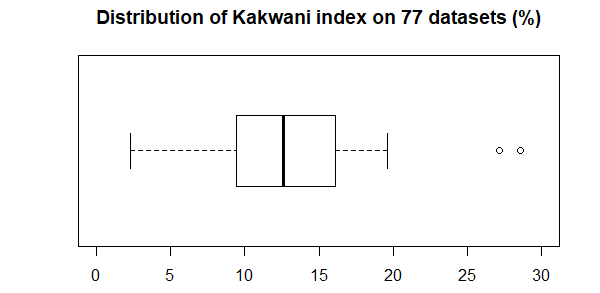
\includegraphics{images/boxplot_kakwani.png}
    \caption{Boxplot of the Kakwani indices}
    \label{fig:kakwani_boxplot}
\end{figure}

Based on the different tax rates that we have computed earlier, we are now able to frame the possible values of the RS index. As summed up in \cref{fig:RS_scenarii}, most values for the Reynolds-Smolensky index will lie between -0.02 and -0.08.
\begin{figure}
	\centering
	\includegraphics[scale=0.8]{"images/18-12 RS_scenarii"}
	\caption{Value of Reynolds-Smolensky index depending on tax rate and Kakwani index}
	\label{fig:RS_scenarii}
\end{figure}

\section{Country and years coverage}
\label{A-datasets}
We select a total of \textbf{216} LIS datasets. 

In \cref{tab:datasets}, countries marked with an \textbf{(R)} are used in the regression pool. For years marked with an *, information on rents is missing.

\begin{tabularx}{\textwidth}{lXX}
        \caption{Country and years used in the study} \\
\hline
Country            & Years with observed data                       & Years with imputed data                                       \\ \hline
Australia \textbf{(R)}      & 2010*                                          & 1989, 1995, 2001, 2003, 2008                                  \\
Austria            &                                                & 1994, 1995, 1997, 2000, 2004, 2007, 2010, 2013                \\
Belgium            &                                                & 1992, 1995, 1997*, 2000                                       \\
Brazil             &                                                & 2006, 2009, 2011, 2013                                        \\
Colombia           &                                                & 2007, 2010, 2013                                              \\
Czech Republic     &                                                & 2004, 2007, 2010, 2013                                        \\
Denmark            &                                                & 1987*, 1992, 2000, 2004, 2007*, 2010*, 2013*                  \\
Dominican Republic & 2007                                           &                                                               \\
Estonia            & 2000                                           & 2004, 2007, 2010, 2013                                        \\
Finland            &                                                & 1987*, 1991, 1995*, 2000*, 2004*, 2007*, 2010*, 2013*         \\
France \textbf{(R)}         & 1984, 1989, 1994, 2000, 2005, 2010             &                                                               \\
Germany            &                                                & 1984, 1989, 1994, 2000, 2004, 2007, 2010, 2013                \\
Greece             &                                                & 2004, 2007, 2010, 2013                                        \\
Guatemala          & 2006, 2014                                     & 2011                                                          \\
Hungary \textbf{(R)}        & 1991, 1994, 1999, 2005, 2007, 2009, 2012       &                                                               \\
Iceland            &                                                & 2004, 2007, 2010                                              \\
India              & 2004, 2011                                     &                                                               \\
Ireland            &                                                & 1994, 1995, 1996, 2000, 2004, 2007, 2010                      \\
Israel             & 2001, 2005, 2007, 2010, 2012                   & 1979*                                                         \\
Italy \textbf{(R)}          & 1995*, 1998*, 2000*, 2004*, 2008*, 2010*, 2014 & 1986*, 1987, 1989, 1991, 1993                                 \\
Japan              &                                                & 2008                                                          \\
Luxembourg         &                                                & 1991, 1994, 1997, 2000, 2007, 2010, 2013                      \\
Mexico             & 2008, 2010, 2012                               & 1984*, 1989*, 1992*, 1994*, 1996*, 1998*, 2000*, 2002*, 2004* \\
Netherlands        &                                                & 1983*, 1987, 2004, 2007, 2010, 2013                           \\
Norway             &                                                & 1979*                                                         \\
Panama             &                                                & 2010, 2013                                                    \\
Paraguay           &                                                & 2010, 2013                                                    \\
Peru               & 2004, 2007, 2010, 2013                         &                                                               \\
Poland \textbf{(R)}         & 2007, 2010, 2013                               & 1986*, 1995*, 1999*, 2004*                                    \\
Russia             & 2000, 2004, 2007, 2010, 2013                   &                                                               \\
Serbia             & 2006, 2010, 2013                               &                                                               \\
Slovakia           &                                                & 2004, 2007, 2010, 2013                                        \\
Slovenia \textbf{(R)}       & 1997, 1999, 2004, 2007, 2010, 2012             &                                                               \\
Spain \textbf{(R)}          & 1980, 1990                                     & 1995, 2000, 2004, 2007, 2010, 2013                            \\
Sweden             &                                                & 2000, 2005                                                    \\
Switzerland        &                                                & 1982*, 1992, 2007, 2010, 2013                                 \\
Taiwan \textbf{(R)}         & 1981, 1986, 1991, 2007, 2010, 2013             & 1995*, 1997*, 2000*, 2005*                                    \\
United Kingdom \textbf{(R)} & 1986, 1991, 1995                               & 1994, 1999, 2004, 2007, 2010, 2013                            \\
United States      &                                                & 1979, 1986, 1991, 1994, 1997, 2000, 2004, 2007, 2010, 2013    \\
Uruguay            &                                                & 2004*, 2007, 2010, 2013                                       \\ \hline
    \label{tab:datasets}
    
\end{tabularx}

